\documentclass{article}
\usepackage[utf8]{inputenc}
\usepackage{graphics}
\usepackage{amsmath}
\usepackage{graphicx}
\usepackage{geometry}
\usepackage{caption}
\usepackage{url}




\title{Software Requirements Specification: Chrome Dino Runner \\ \bigskip \large SFWRENG 3XA3 Project \\ \bigskip \large Team Number: L03 Group 1 \\ \large Team Name: ``Team Rex'' }

\author{Chelsea Maramot \\ maramotc \\ \\ Anjola Adewale \\ adewaa1 \\ \\ Sheridan Fong \\ fongs7 }

\date{February 11 2022}

\begin{document}

\maketitle
% section 1: Project Drivers ---------------------------
\section{Project Drivers}
\subsection{The Purpose of the Project}
The current pandemic has abruptly disrupted the entertainment sector, and now people are seeking entertainment within the comfort of their homes. An example of an at-home entertainment solution is video games. We aim to provide home entertainment by redesigning the classic Chrome T-Rex dinosaur game. We plan to improve its user-friendliness and interactivity while maintaining the game’s basic functionality. The game's development will follow the software development process and be implemented in python using the PyGame library. The entire process will be documented and tested using the unit test framework. 
\subsection{The Stakeholders}
\subsubsection{The Client}
The clients for this project are the course instructor of SFWRENG 3XA3, Dr. Ashgar Bokhari, and the teaching assistants (TAs), Stephanie Koehl, Veersah Palanichamy and Abdul Rab Mohammed. The clients will provide project requirements, deliverables and deadlines. They will also provide guidance when necessary and evaluate the project with respect to the requirements in the SRS document. 
\subsubsection{The Customers}
The customers for this project are individuals who are interested in playing Chrome-Dino. The project does not explicitly target a demographic but is rather designed as a general-purpose entertainment source. The project is designed for anyone with the game's required software, such as Python and the PyGame library. 
\subsubsection{Other Stakeholders}
All members of group 1 are stakeholders of this project. We are all responsible for the development process, such as implementing, testing, and documenting the project. Group 1 members all care for the project's success and are responsible for maintaining the repository. Developers that fork the repository and continue the project's development are also stakeholders as they will be continuing the project and are interested in the project's success



% Section 2: Project Constraints 
\section{Project Constraints}
are restrictions on the product due to the budget or the 
time available to build the product
    \subsection{Mandated Constraints}
    \subsubsection{Solution Design Constraints}
    Description: The game (an executable file) must be able to run on any machine running on Windows 7 or newer, macOS 10.12 
    Rationale: Most computer users already use systems with these specification and so the users will not need to purchase a new system.
    Fit criterion: The game will be developed into an executable file that will be made to run on Windows & or newer, macOS Sierra 10.12 or newer or Linux Ubuntu or newer4
\subsubsection{Implementation Environment of the Current System}
N/A
\subsubsection{Partner of a Collaborative Application}
N/A
\subsubsection{Off-the-Shelf Software}
N/A
\subsubsection{Anticipated Workable Environment}
N/A
\subsubsection{Schedule Constraints}
Description: This project must follow the project schedule outlined in the Gantt chart and the Task Section.
Rationale: This is because, the project must be completed prior to the end of the course a strict pre-defined plan must be followed. This is also so to ensure that all deliverable are submitted by their due dates
Fit Criterion: All deliverable contained within this project must completed and submitted by April 12, 2022 

Due to the time constraints on this project(3 months), this project needs to follow a predefined plan in order to ensure it's completion in an organized manner.
\subsubsection{Budget Constraints}
\subsubsection{Enterprise Constraints}
\subsection{Naming Conventions and Terminology}
\subsection{Relevant Facts and Assumptions}
\subsubsection{Facts}
\subsubsection{Assumptions}



% Section 3: Functional Requirements
\section{Functional Requirements}

\subsection{The Scope of the Work and the Product}

\subsubsection{The Context of the Work}
% come back to and insert picture properly 
\begin{figure}
    \centering
    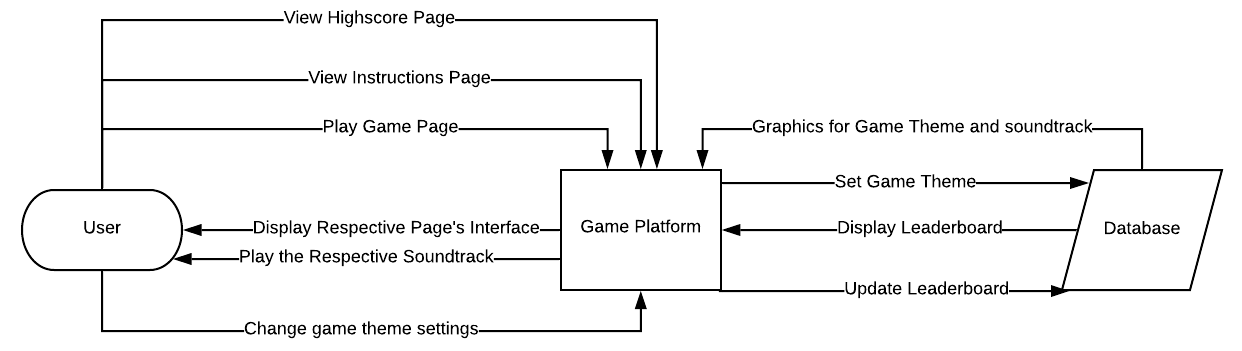
\includegraphics{context_diagram.png}
    \caption{Caption}
\end{figure}

\subsubsection{Work Partitioning}


\subsubsection{Individual Product Use Cases}

\subsection{Functional Requirements}




% section 4 -----------------------
\section{Non-Functional Requirements}
    \subsection{Look and Feel Requirements}
        \subsubsection{Appearance Requirements}
        LFX. The user interface consist of essential components relevant to the game.
        \subsubsection{Style Requirements} 
    	LFX. The product shall maintain the 90's arcade appearance.\\
    	LFX. The product shall be designed according to the extra themes developed.
   
\subsection{Usability and Humanity Requirements}
    \subsubsection{Ease-Of-Use Requirements}
    UHX. Game can be controlled using two methods, arrow keys and AWSD keys.\\
    UHX. The game must have a simple menu page where game settings can be accessed.\\
    UHX. The game can be used by people intuitively, no training needed and at a maximum basic English level.
    
    \subsubsection{Personalization and Internationalization Requirements}
    PIx. The product shall only be used in English.
    PIX. The user can adjust the theme of the game based on their preferences.
    
    \subsubsection{Learning Requirements}
    LRx. The game will be used without receiving training before using it.\\
    LRx. The game must contain basic instructions within the main menu page.

    \subsubsection{Understandability and Politeness Requirements}
    UPx. The game shall encompass a level of abstraction from the user.\\
    UPx. The game shall use common control keys to play the game.\\
    UPx. The game will include universal symbols and words that are naturally understood by the user community.
    
    \subsubsection{Accessibility Requirements}
    ARx. The game shall be playable for those with colour blindness.
    
\subsection{Performance Requirements}
    \subsubsection{Speed and Latency Requirements}
    PEX. Scores must be uploaded to the leader board in less than 10 seconds.\\
    PEx. The interface must have a maximum response time of 2 seconds.
    PEx. The game shall update the new status parameters within 5 minutes of user input.

    \subsubsection{Safety-Critical Requirements}
    N/A
    
    \subsubsection{Precision or Accuracy Requirements}
    PEx. Integer whole number scores must be uploaded appropriately and displayed on the screen\\
    PEx. Leader board shall be updated according to the top integer score
    
    \subsubsection{Reliability and Availability Requirements}
    N/A

    \subsubsection{Robustness or Fault-Tolerance Requirements}
    N/A
    
    \subsubsection{Capacity Requirements}
    PEx. The game shall only be available to a single player\\
    PEx. The game shall allow a maximum of 3 users stored in the leader board.
    
    \subsubsection{Scalability or Extensibility Requirements}
    PEx. Developers shall be able to add new features, such as themes, without compromising basic functionalities of the game. 
    
    \subsubsection{Longevity Requirements}
    PEx. The game must maintain functionality with existing software until Spring 2022.


\subsection{Operational and Environmental Requirements}
    \subsubsection{Expected Physical Environment}
    PEx. The game can be played with full functionality without internet connection.\\
    PEx. The game can be played within any computer operating system (i.e. Linux, Windows)
    
\subsection{Requirements for Interfacing with Adjacent Systems}
    \subsubsection{Productization Requirements}
    PEX. The game shall be distributed to user computers as a .EXE file.
    PEX. The game shall be installed without the use of separately printed instructions.
    
 \subsection{Release Requirements}
    PEX. The game will be released by April 5, 2021.
    
 \subsection{Maintainability and Support Requirements}
    \subsubsection{Maintenance Requirements}
    \subsubsection{Supportability Requirements}
    \subsubsection{Adaptability Requirements}
    
\subsection{Security Requirements}
    \subsubsection{Access Requirements}
    \subsubsection{Integrity Requirements}
    \subsubsection{Privacy Requirements}
    \subsubsection{Audit Requirements}
    \subsubsection{Immunity Requirements}
    
\subsection{Cultural and Political Requirements}
    \subsubsection{Cultural Requirements}
    \subsubsection{Political Requirements}    
    
\subsection{Legal Requirements}
    \subsubsection{Compliance Requirements}
    \subsubsection{Standards Requirements}    
\subsection{Health and Safety Requirements}

%section 5
\section{Project Issues}
\subsection{Open Issues}
\subsection{Off-the-Shelf Solutions}
\subsection{New Problems}
\subsection{Tasks}
\subsection{Migration to the New Product}
\subsection{Risks}
\subsection{Costs}
\subsection{User Documentation and Training}
\subsubsection{Documentation}
\subsubsection{Training}
\subsection{Waiting Room}
\subsection{Ideas for Solutions}
\end{document}
